\begin{frame}{Travail réalisé : Maillage quadrilatère 2D}
    \centering
    \begin{enumerate}
        \item Une seule géométrie en entrée :
        \begin{itemize}
            \item Champ de repère adapté à des modèles CAO.
            \item Quantification sans recalcul de paramétrisation.
            %\item Implémentation web (ThreeJS + WebAssembly) : \url{ddesobry.github.io/quadmesher.html}
            \only<2-3>{
                \item Correction des problèmes de non-intégrabilité.    
                \item 100\% de réussite sur la b.d.d Mambo [\cite{ledoux_mambo_2019}]
            }
        \end{itemize}
        \only<3>{
            \item Maillage quad pour une simulation de déformation :
            \begin{itemize}
                \item Alternance automatisée entre simulation et maillage. 
                \item Valences de bord adaptées aux géométries de déformation.
                \item 3 simulations industrielles réalisées automatiquement. 
            \end{itemize}
        }
    \end{enumerate}
    \only<1>{
        \vspace{2em}
        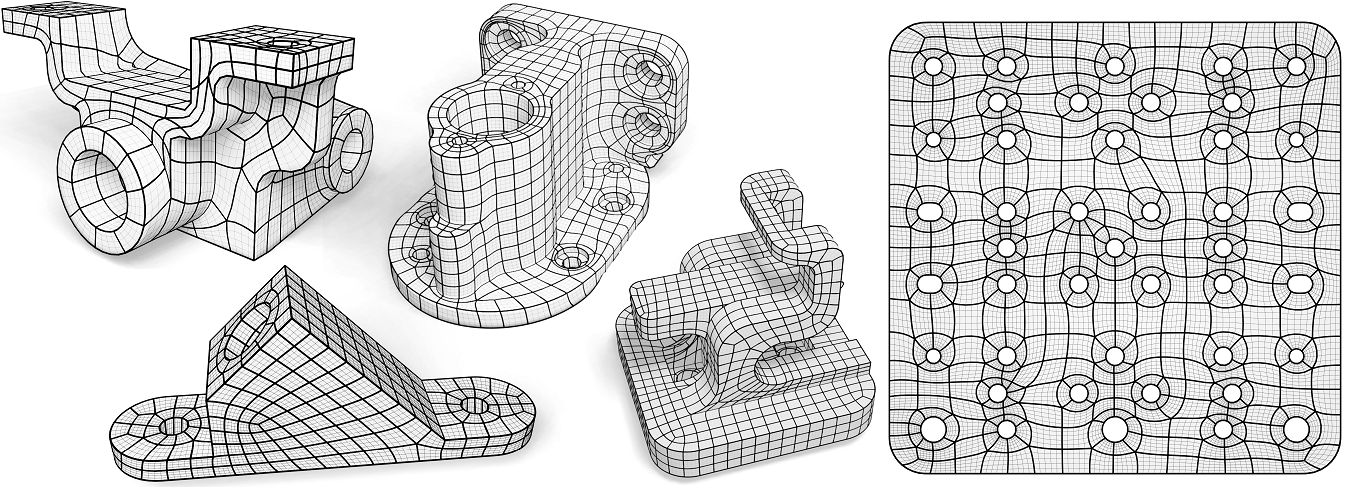
\includegraphics[width=\linewidth]{img/quadsimu/5_meshes_min.png}
    }
    \only<2>{
        %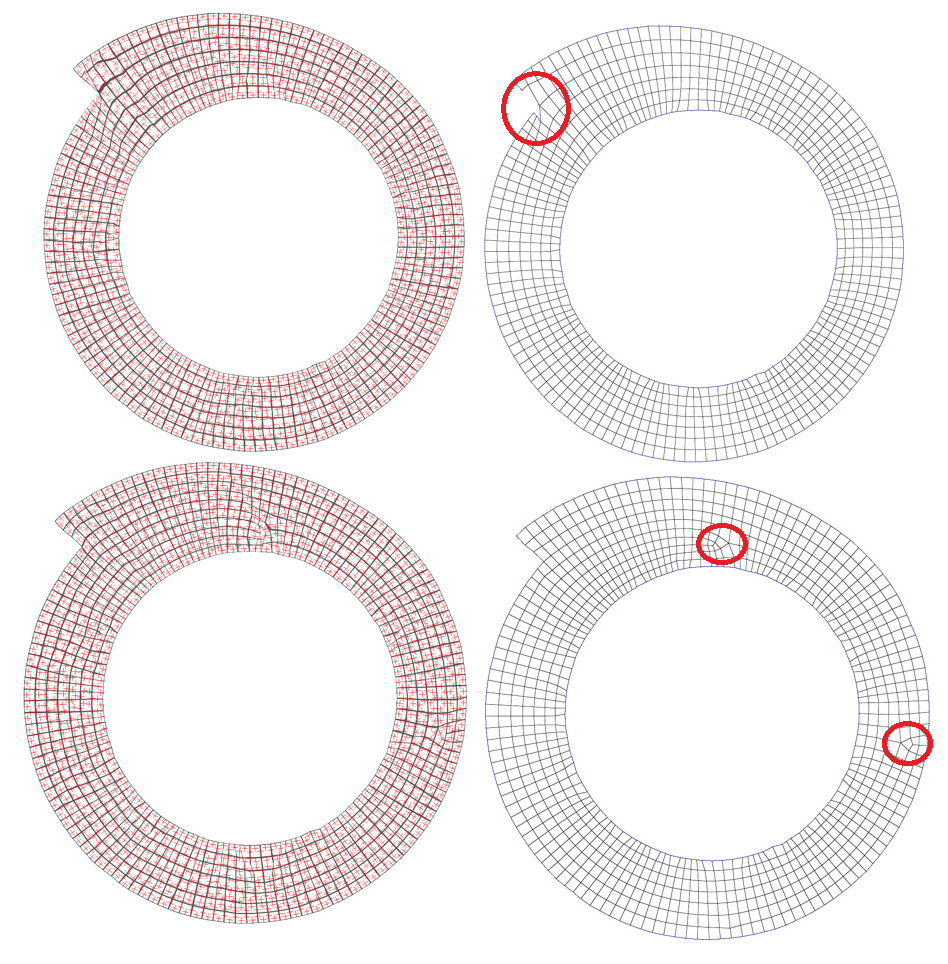
\includegraphics[width=.49\linewidth]{img/quadsimu/solve_sharkanulus_2}
        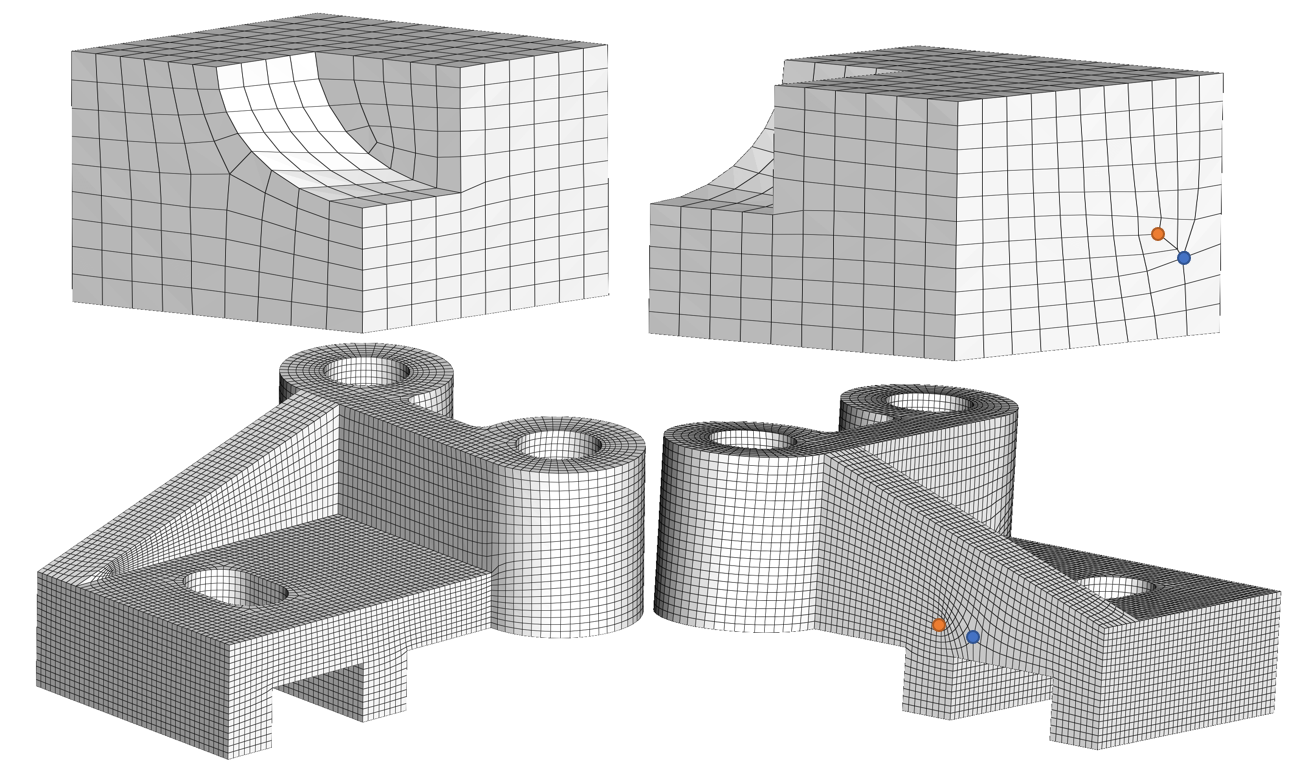
\includegraphics[width=.7\linewidth]{img/quadsimu/sharkanulus_mambo}
    }
\end{frame}
    
\iffalse
\begin{frame}{Travail réalisé : Maillage hexaédrique 3D}
    \begin{enumerate}
        \item Réparation incrémentale des graphes de singularité
        \item Champ de repère avec singularités de bord imposées.
    \end{enumerate}

    \begin{itemize}
        \item "[\cite{ledoux_mambo_2019}]" / \cite{ray_practical_2016} / \cite{ray_practical_2016} + (1) / \cite{ray_practical_2016} + (2)
        \item "Basique" (74 modèles) / 18\% / 40\% / 69\%
        \item "Simple" (29 modèles) / 0\% / 21\% / 34\%
        \item "Medium" (9 modèles) / 0\% / 0\% / 0\%
    \end{itemize}
\end{frame}
\fi

\begin{frame}{Travail réalisé : Maillage hexaédrique 3D}
    \small
    \centering
    \begin{enumerate}
        \item Réparation de graphe de singularité de champ de repère \label{enum:reparation}
        \item Champ de repère avec singularités de bord imposées. \label{enum:champ}
    \end{enumerate}
    %L'algorithme de calcul de champ de repère est \cite{ray_practical_2016}
    \begin{table}
    \centering
    \scriptsize
    \begin{tabular}{|l|c|c|c|}
    \hline
    Base de données & [\cite{ray_practical_2016}] & + (\ref{enum:reparation}) & + (\ref{enum:champ}) \\
    \hline
    Mambo-Basique & 18\% & 40\% & 69\% \\
    \hline
    Mambo-Simple & 0\% & 21\% & 34\% \\
    \hline
    Mambo-Medium & 0\% & 0\% & 0\% \\
    \hline
    \end{tabular}
    \end{table}
    \% de maillages réussis  en fonction de l'utilisation de (\ref{enum:reparation}) et (\ref{enum:champ})
    \only<1>{
        \begin{columns}[T] % align columns
            \centering
            \begin{column}{.45\linewidth}
                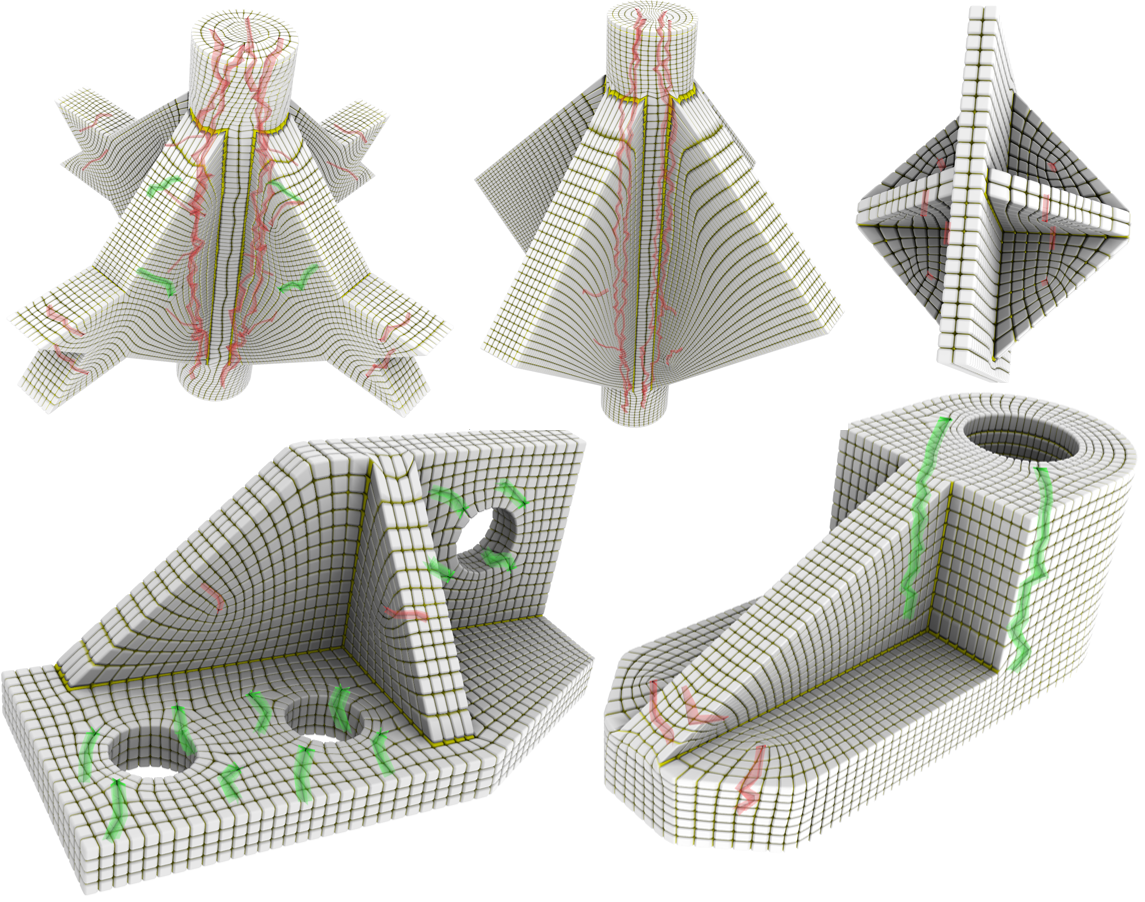
\includegraphics[width=\linewidth]{img/hexmeshing_ff/resultats_3.png}
            \end{column}
            \begin{column}{.45\linewidth}
                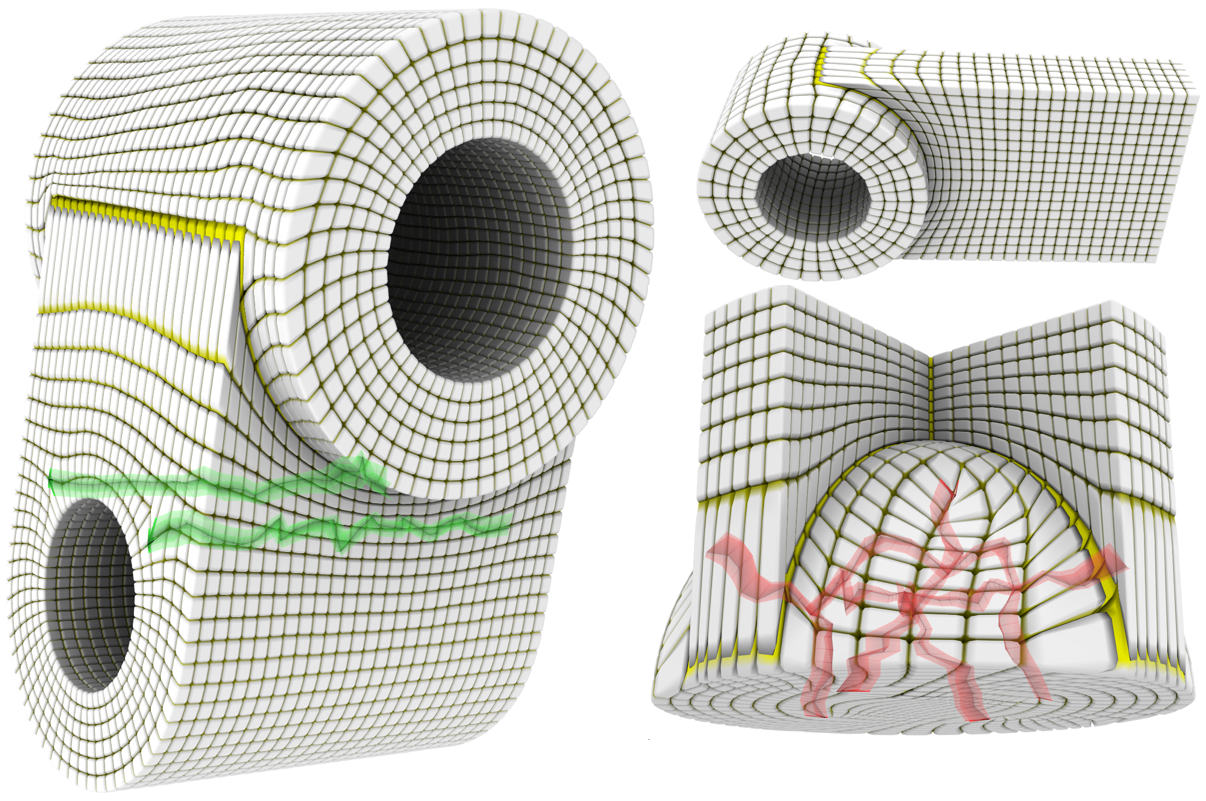
\includegraphics[width=\linewidth]{img/hexmeshing_ff/prescribed_valences.png}
            \end{column}
        \end{columns}
    }
\end{frame}

\iffalse
\begin{frame}{Perspectives}
    \textbf{Maillage quadrilatère:}
    \begin{itemize}
        \item Correction champ de repère : Résoudre les problèmes de non-intégrabilité sans trop affecter la qualité.
        \item Intégrabilité champ de repère : Optimiser le placement des singularités sans trop affecter les performances.
    \end{itemize}
    \pause
    \textbf{Maillage hexaédrique:}
    \begin{itemize}
        \item Initialisation champ de repère : Méthode automatique pour déterminer des valences sur le bord valides.
        \item Correction champ de repère : Méthode de correction robuste des graphes de singularités intérieurs [\cite{liu2023locally}].
        \item Quantification rapide : Résoudre le problème de quantification par une méthode gloutonne comme en 2D.
    \end{itemize}
\end{frame}
\fi

\begin{frame}{Perspectives}
    \scriptsize
    \begin{table}
        \centering
        \begin{tabular}{|l|c|c|c|}
        \hline
        Base de données & [\cite{ray_practical_2016}] & + (\ref{enum:reparation}) & + (\ref{enum:champ}) \\
        \hline
        Mambo-Basique & 18\% & 40\% & 69\% \\
        \hline
        Mambo-Simple & 0\% & 21\% & 34\% \\
        \hline
        Mambo-Medium & 0\% & 0\% & 0\% \\
        \hline
        \end{tabular}
    \end{table}
    \small
    \textbf{Pistes d'amélioration de la paramétrisation globale 3D :}
    \begin{enumerate}
        \item Correction champ de repère : Méthode de correction robuste des graphes de singularités intérieurs [\cite{liu2023locally}].
        \item Initialisation champ de repère : Méthode automatique pour déterminer des valences sur le bord valides.
        \item Quantification 3D sans recalcul de paramétrisation : Décimation du maillage tétrahédrique d'entrée et résolution gloutonne.%Résoudre le problème de quantification sur un maillage tétraédrique décimé.
    \end{enumerate}
\end{frame}